%\chapter{Bericht}
%==========================
\chapter{Aufgabe}
%==========================
Mobile Serviceroboter stellen in verschiedensten Anwendungsbereichen eine vielversprechende Zukunftstechnologie dar. 
Dazu gehören beispielsweise fahrerlose Transportfahrzeuge (FTF), wie sie derzeit bereits in Intralogistik und Produktion zum Einsatz kommen, autonome Reinigungs- und Inspektionsroboter oder auch autonome Straßenfahrzeuge, welche sich ebenfalls in dieser Kategorie einordnen lassen. 
Schlüsseltechnologie dieser Systeme ist die autonome Navigation. 
Durch diese werden die mobilen Systeme befähigt, sich selbstständig durch die Umgebung, in der sie operieren, zu bewegen. 
Kernkomponenten autonomer Navigation sind die Lokalisierung des Roboters, die Wahrnehmung von Objekten und Hindernissen sowie die Bewegungsplanung.
Die Lokalisierung eines Roboters basiert in der Regel auf der Auswertung von Sensormessungen und Abgleich mit einer Umgebungskarte. 
Für die Generierung und Aktualisierung von Umgebungskarten spielen sogenannte SLAM(Simultaneous Localization and Mapping)-Verfahren eine bedeutende Rolle.
Das Fraunhofer IPA untersucht derzeit in verschiedenen Projekten die Anpassung und Weiterentwicklung bestehender Lokalisierungskonzepte. 
Der Fokus liegt dabei auf der Lokalisierung für Multi-Robot-Systeme (Cooperative SLAM) sowie der Langzeit-Lokalisierung und Langzeit-Kartierung in dynamischen Umgebungen (Lifelong Localization).

Meine aufgaben bestanden haupsächlich darin zu testen wie gut sich autonome Navigation auf Lowcost systemen betreiben lässt.

Die Arbeiten fanden unter Nutzung des \emph{Robot Operating System} (ROS)\cite{Quigley-ICRA-2009} statt.
Im Detail beschäftigte ich mit den folgenden Themen:

\begin{itemize}
\item Einrichten des \emph{Robot Operating System} auf einem Raspberry Pi v2 und einem Odroid XU4
\item Testen der Lokalisierungs- und Bahnplanugssoftware mit dem Robopeak Lidar
\item Updaten der Software \emph{slam\_karto} fur den Betrieb auf Odroid XU4
\item Verändern eines layers der Costmap des move\_base Packets von \emph{Robot Operating System}
\end{itemize}

%==========================
\chapter{Problemlösung}
%==========================
\section{ROS auf Embedded Systemen}
%==========================
Meine erste Aufgabe war das einrichten des \emph{Robot Operating System}, kurz \emph{ROS}, auf einem Raspberry Pi.

ROS ist ein Open Source Projekt, was im Bereich Robotik weit verbreitet ist.
Es handelt sich hierbei um ein Framework zur flexiblen Erstellung von Roboter-Steuerungen. Es bietet dem Benutzer ein Netzwerk an mit dem er beliebig viele Komponenten verkoppeln kann. Ausserdem beinhaltet das Framework eine Vielzahl von Komponenten die direkt verwendet werden können oder angepasst werden können.
Die Komponenten heißen \Glspl{node} und können in C++ oder Python geschrieben werden. Diese kommunizieren über sogenannte Topics die man sich als Datenkanäle vorstellen kann. Danz ganze wird von einem \Gls{master} gesteuert der die anfragen der einzelnen \Glspl{node} entgegennimmt und sie verarbeitet. 
Seit der ROS Version Groovy Galapagos (Released 31.12.2012) ist Catkin das standard Buildsystem das aus dem Source Code ausführbare Dateien macht. Dieses basiert auf dem Buildsystem CMake was das Kompilieren von Großen Software-Ketten sehr vereinfacht. CMake sucht selbständig den Pfad von ausführbaren Dateien und Libraries und schreibt die MAKE-Files für den Compiler (GCC). Dieses System wird von \Gls{catkin} benutzt um die Dateien in sogenannte \Glspl{catkin workspace} zu sortieren. Ein \Glspl{catkin workspace} besteht aus Source Space, Build Space, Devel Space und Install Space.
Der Source Space enthält den Quellcode der verschiedenen Software-Packete und jeweils eine Datei namens CMakelists.txt in der die Abhängigkeiten und andere spezifische Einstellungen jedes Packets festgelegt sind. 
Der Build Space dient als Zwischenspeicher für den Kompiliervorgang für Catkin und Cmake.
Im Development (Devel) Space werden die Kompilierten Dateien abgelegt und zum ausführen bereitgestellt. So können die ausführbaren Dateien getestet werden bevor sie durch das installieren im Install Space enden.
\Gls{catkin} ermöglicht auch das Verketten von \Glspl{catkin workspace} um somit ganze Software Strukturen einfach in ein Projekt einzubinden. Man kann z.B. die Dateien die man bearbeitet in einen \Gls{catkin workspace} legen den man mit einem weiteren \Gls{catkin workspace} mit fertigen Programmen verknüpft. So geht der Kompiliervorgang der bearbeiteten Quelldateien wesentlich schneller da nicht alle Packete auf Änderungen überprüft werden.

%==========================
\subsection{Raspberry Pi}
%==========================



%==========================
\subsubsection{Hardware}
%==========================

 Das Raspberry Pi ist ein lowcost Embedded System (Einplatinencomputer) welches von der Raspberry Pi Foundation in Großbritannien entwickelt wurde.
 Das System wird von einer 900MHz quad-core ARM Cortex-A7 CPU angetrieben und verfügt über 1 GB Arbeitsspeicher.
 Außerdem lässt das Board sich über einige Schnittstellen erweitern: 4x USB 2.0, 40 GPIO Pins, Ethernet, ein Camera interface (CSI), ein Display interface (DSI) und ein analogen Audio Port. Als speicher dient eine SD-Karte.
 Dank dem niedrigen Preis (unter 40 Euro) und dem guten Preis-Leistungsverhältnis ist das Raspberry Pi einer der beliebtesten und verbreitetsten Single Board PCs.
 
%==========================
\subsubsection{Software}
%==========================

Als Betriebssystem diente dem Raspberry Pi in meinem fall Raspbian Wheezy. Hierbei handelt es sich um ein auf Debian ARM hard-float basierenden Linux System. Es gibt sehr viele alternativen aber Raspbian ist von den Herstellern entwickelt und am meisten verbreitet, daher ist es für die Hardware-Komponenten optimiert und nutzt deren leistung am besten aus.
Raspbian benutzt, wie Debian, den Packetmanager APT um das installieren von Software zu vereinfachen. APT bezieht die vorkompilierten Packete aus sogenannten Repositories die in der Datei \emph{sources.list} auflistet sind und verändert werden können. 

%==========================  
\subsubsection{ROS-Installation}
%==========================  

Der Prozessor des Raspberry Pi 2 basiert auf der ARM Architektur, ROS wird aber nicht standardmäßig in Packetform für ARM bereitgestellt. Daher mussten sämtliche Packete aus den Source-Dateien kompiliert werden. Bei diesem Vorgang traten einige Schwierigkeiten auf da ich mich erst mit Linux und dem GCC Compiler vertraut machen musste und viele Abhängigkeiten der Packete auch kompiliert werden mussten.

Als erstes habe ich das Betriebssystem Raspbian als img Datei (raw disk image file, die kopie eines Laufwerks) bezogen und mittels dem Unix-Befehl DD auf die SD-Karte geschrieben. Nachdem das Raspberry Pi erfolgreich von der Speicherkarte gestartet war, habe ich den Quellcode des des gesamten ROS Systems in den Source Space geladen. Nachdem alle nicht in den Repositories vorhandenen Abhängigkeiten aus dem Source Code erstellt wurden habe ich die restlichen mit dem ROS-Tool \emph{rosdep} installiert. Dieses Tool durchsucht sämtliche \Glspl{package} in einem \Gls{catkin workspace} auf Abhängigkeiten und installiert diese automatisch mittels APT.
Somit war alles vorhanden um ROS zu kompilieren. Beim ersten Versuch gab es einen Fehler bei dem Packet Collada den ich mittels \Gls{patch file} behoben habe. 
Danach lief der Kompiliervorgang problemlos durchm, brauchte aber aufgrund der schwachen Hardware einige Stunden.

%==========================  
\subsubsection{Installation der Navigations Software des IPA}
%==========================  

Nachdem der erste roscore (\Gls{master}) erfolgreich gestartet war ging es weiter mit der Installation der Software für Lokalisierung und Navigation des \emph{Fraunhofer IPA}.
Das \emph{IPA} verwendet für die Verwaltung des Codes das Versioning Tool \emph{git} in Verbindung mit dem Online-Dienst \emph{GitHub}. 
\emph{Git} ist ein Versionsverwaltungssystem das von Linus Torvalds im April 2005 entwickelt wurde. Es vereinfacht den Entwicklungsprozess und die Kollaboration zwischen Programmierern ungemein. Jede Änderung im Quellcode wird in \Glspl{commit} festgehalten die aufeinander aufbauen. Diese Ketten aus \Glspl{commit} werden \Glspl{branch} genannt und können beliebig verzweigt werden. So kann beispielsweise auf einem \Gls{branch} der aktuelle stand eines Programms bearbeitet werden und auf einem Zweig eine neue Funktion getestet werden ohne den aktuellen Stand zu beeinflussen.

\begin{figure}[ht]
\begin{center}
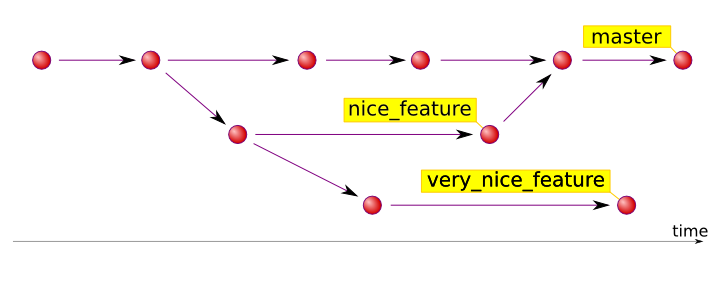
\includegraphics[width=0.8\textwidth]{git-branches}
	\NIcaption{git branches}{Auf dem Bild ist eine Beispiel Anordnung von Branches zu sehen. Der nice\_feature branch wurde erst ge\emph{forkt} und dann wieder ge\emph{merged} nachdem das feature fertigestellt wurde.}
  \label{git branches}
\end{center}
\end{figure}

Um den Code zu teilen wird der Online-Dienst GitHub verwendet. Dort legt man eine Kopie der localen Daten an sodass andere darauf zugreifen können. Ähnlich dem \Gls{branch}-system macht der User ein \Gls{fork} von einem \Gls{git repository}, auf dem der aktuelle stand der zu entwickelnden Software liegt. Somit hat der User einen parallelen Stand an dem er arbeitet und z.B. nach Abschließen eines \Gls{feature}s stellt er eine Anfrage an den Administrator des Repository  um seinen Stand in die Software zu \Gls{merge}n. Das nennt man einen \Gls{pull request}.

Nachdem ich mit in das git-System eingearbeitet hatte, habe ich den \Gls{source code} aller \Glspl{package} die für die Lokalisierung und für die Bahnplanung erforderlich sind aus den entsprechenden \Glspl{git repository} in den Source Space eines neuen \Gls{catkin workspace}s geladen.
Beim ersten durchlauf von \Gls{rosdep} traten die ersten großen Probleme auf. Neben \emph{libcrypto++} wurden \emph{OpenCV} und die \emph{Point Cloud Library} als \Glspl{dependencie} benötigt. Nach einer kurzen Recherche fand ich heraus das letztere zwei sich zwecks mangelndem Arbeitsspeicher nicht so leicht auf dem \emph{Raspberry Pi} kompilieren lassen. Ich fand jedoch eine vorkompilierte Version in den Software Repositories von Raspbian Jessie das zu dem Zeitpunkt noch im Beta-Stadium war. So fügte ich diese in die \emph{sources.list} von APT ein und installierte die notwendigen Software-Packete.
Leider wurden somit bei dem nächsten System-Update einige Programme aus den Wheezy Repositories ersetzt mit Versionen aus den Jessy Repositories. Das führte dazu das APT diese Programme nicht mehr als \Glspl{dependencie} erkannte und somit nicht mehr funktionierte. Nach einigen Nachforschungen entschied ich mich das gesamte Betriebssystem neu zu installieren da dies die schnellste Lösung für das Problem darstellte.
Nachdem ich wieder auf dem vorherigen stand angelangt war entschied ich mich keine externen Software Repositories mehr einzubinden da ich die folgen zu genüge erfahren habe.
Nach einer weiteren Suche stieß ich auf das sogenannte \emph{Cross Compiling}. Dieses ermöglicht Programme für eine andere Architektur zu kompilieren, z.B. aus dem \Gls{source code} der \emph{Point Cloud Library}, auf einem herkömmlichen PC eine ausführbare Datei für das Raspberry Pi herzustellen. Da das Vorgehen recht umständlich war beschloß ich noch einen schritt weiter zum \emph{Distributed Compiling} zu machen. Hierfür richtete ich den \emph{Distcc Client} auf Raspberry Pi und den \emph{Distcc Server} auf dem PC ein. Der \emph{Client} ersetzt den GCC Compiler und fängt somit alle Aufrufe auf diesen ab und schickt die zu kompilierenden Dateien an den Server auf dem PC. Dieser schickt nach erfolgreichem Kompiliervorgang die ausführbare Datei über das Netzwerk zurück. 
Das ermöglichte letzendlich das erfolgreiche installieren der fehlenden \Glspl{dependencie} und ersparte bei jedem folgenden Kompiliervorgang viel Zeit.
Das nächste Problem trat beim einbinden des \emph{ipa\_licence\_verifier} auf da dieser auf einer vorkompilierten Library basiert die für die Architektur \emph{x86-64} bestimmt ist. Bei Nachfrage bei den Betreuern erfuhr ich das es in einem anderen Repository den \Gls{source code} zu dieser Library gibt. Leider lies sich dieser auch nicht problemlos Kompilieren da er auf Harware Register zugreift die auf dem \emph{Raspberry Pi} nicht verfügbar sind. 
Daher entfernte ich provisorisch den unkompatiblen Code da er in naher Zukunft eh überholt werden sollte.
Somit wurden die gesamten \Glspl{package} erfolgreich kompiliert und ich konnte mit dem testen anfangen.

%==========================  
\subsubsection{Testen der Navigations Software des IPA}
%==========================  

Beim ersten starten der Navigations und Lokalisierungs Software wurde sehr schnell klar, dass das Rasperry Pi nicht über genügend Leistung verfügt.
In ROS kann man die Frequenz der Aufrufe einer Funktion festlegen, aber das Raspberry Pi erziehlte weniger als die Hälfte der Wiederholungen.
Auf der Suche nach einer Lösung bin ich auf Hardware-spezifische Compiler Flags gestoßen. Diese ermöglichen es den Binary Code der Ausführbaren Dateien auf den Prozessor abzustimmen und somit eine deutliche Leistungssteigerung zur Folge haben.
Nach vielem recherchieren und testen fand ich eine Kombination mit der die Lokalisierung flüssig lief. Bei der erwarteten Wiederholrate lastete diese den Prozessor des Raspberry Pis sogar nur zur Hälfte aus. Die Navigation lief jedoch trotz dieser Optimierung nicht einwandfrei, daher schaute ich mich nach leistungsstärkerer Hardware um.

%==========================
\subsection{Odroid XU4}
%==========================

%==========================
\subsubsection{Hardware}
%==========================

Das Odroid war zu dem Zeitpunkt das leistungsstärkste Embedded System unter 100 Euro. Dieses Board hat für den Preis von 80 Euro eine herausragende Performance.
Es wird von einer einem Prozessor mit Cortex-A15 \& Cortex-A7 big.LITTLE Architektur. Dieser verfügt über 4 Leistungsstarke Rechenkerne mit einer Taktfrequenz von 2 GHz und 4 Stromsparenden mit 1.4 GHz. Diese Technologie wurde für den mobilen Einsatz entwickelt, z.B. für Smartphones und Tablets.
Ausserdem sind auf dem Board 2 GB LPDDR3 RAM und ein Mali-T628 MP6 Grafikkern verbaut. Externe geräte lassen sich über die 2 USB 3.0 Ports und den USB 2.0 Port anschließen. Außerdem verfügt das Board über einen Ethernet und einen HDMI Anschluss.
Als Speicher dient dem Odroid eine SD-Karte oder ein eMMC Modul.

%==========================
\subsubsection{Software}
%==========================

Beim Betriebssystem viel die Wahl auf Ubuntu 14.04 for ARM mit einem von Hardkernel (der Hersteller des Odroids) zu verfügung gestellten Kernel der die big.Little Architektur unterstützt.
Dieses bietet im vergleich zu Raspbian einige Vorteile, hauptsächlich die verwendung der Offiziellen Ubuntu Packetquellen die bedeutend mehr Software enthalten.

%==========================  
\subsubsection{ROS-Installation}
%==========================

Die meisten ROS-Packete sind in den Ubuntu-Packetquellen vorhanden aber ich habe mich, da ich bereits gelernt hatte wie das Vorgehen ist, entschlossen diese aus dem \Gls{source code} zu generieren da sie so für die Hardware des Odroids optimiert werden konnten. 
Als erstes richtete ich das Distributet Compiling System, das ich schon auf dem Raspberry Pi erfolgreich benutzt hatte , ein. Anfangs funktionierte es nicht da ich auf dem Odroid eine andere Version zu der auf dem PC installierte. Nach einigem Kopfzerbrechen kompilierte ich die neueste Version von der Entwicklerseite und dann funktionierte es.
Bei der Installation von ROS tritten keine Großen Probleme auf und ich konnte nach kurzer Zeit den ersten \Gls{master} starten.

%==========================  
\subsubsection{Installation der Navigations Software des IPA}
%==========================

Wie schon beim Raspberry Pi, lud ich den \Gls{source code} der Packages aus den jeweiligen \Glspl{git repository} runter und Kompilierte alles mit dem Befehl \emph{catkin\_make}. Schon hier konnte man einen Großen Unterschied der Performance des Odroids im Vergleich zum Raspberry Pi sehen.

%==========================  
\subsubsection{Testen der Navigations Software des IPA}
%==========================  

\begin{figure}[ht]
\begin{center}
\includegraphics[height=0.25\textheight,keepaspectratio]{ipa_navigation}
	\NIcaption{Lokalisierung und Navigation}{Hier sehen sie die Visualisierung der Lokalisierung und der Navigation in dem Visualisierungstool von ROS, \Gls{rviz}.}
  \label{Lokalisierung und Navigation}
\end{center}
\end{figure}

Beim ersten Start stellte ich fest, dass die Navigations- und Lokalisierungs Software auf dem Odroid sehr gut lief. Die Aktualisierung der Position und der berechneten Bahn zum Zielpunkt erfolgte augenscheinlich mit der gleichen Frequenz wie auf dem PC.

Da eine augenscheinliche Betrachtung der Performance keine aussagekräftige Auswertung darstellt, habe ich das System auf Hardwareauslastung getestet. 

Zu diesem zweck habe ich einen Rosnode erstellt der die CPU Auslastung angegebener Prozesse ausliest. Es können beliebig viele Prozessnamen der zu überprüfenden Nodes als Argumente beim aufruf des \Gls{node}s übergeben werden und das Programm liest dann die Timing-Werte aus den entsprechenden Dateien aus dem /proc Ordner aus. Diese Timing-Werte entsprechen der Dauer der belegung der CPU durch den Prozess. Durch Vergleich dieser werte mit der gesamten Zeit zwischen den Aufrufen kann man die CPU Last berechnen. 
Die berechneten Prozentualwerte werden in ein passend erstellten ROS Message eingetragen und über ein Topic versendet. Dieser \Gls{message} beinhaltet ein Double wert mit der Gesamtauslastung und ein Array aus Double werten mit den berechneten Auslastungen der überwachten Prozessen in der Reihenfolge wie sie beim start des Nodes übergeben wurden. Der große Vorteil dieser Methode ist das sich die Auslastung so gemeinsam mit den Positions- und Covarianz-Daten aufnehmen lassen.
Dies habe ich mittels dem ROS-Utility \emph{rosbag} gemacht. Dieses ermöglicht das synchrone aufnehmen und wieder abspielen des Inhalts beliebiger \Glspl{topic}. 

Nachträglich habe ich die Aufgenommenen \Gls{rosbag}-Dateien in \emph{csv}-Dateien umgewandelt um sie anschliessend zu plotten. Mein Betreuer riet mir \emph{GnuPlot} zu diesem Zweck zu verwenden, so erarbeitete ich mir die Grundkenntnisse um dieses Utility zu verwenden.
Mit \emph{GnuPlot} ist es nicht nur möglich vorhandene Daten zu plotten sondern auch diese zu manipulieren und beliebige berechnungen vor der Darstellung zu machen. 
Die gesamten Operationen können in \emph{GnuPlot}-Dateien abgespeichert werden, das ermöglicht das einfache weitergeben der Plots ohne vorher den Zoomfaktor und die Auflösung festlegen zu müssen.

Das Ergebnis dieser Tests bestätigte die vorherige Betrachtung. Die Navigations-Software benötigt weniger als die hälfte der auf dem Odroid vorhandenen Resourcen und läuft somit einwandfrei.

\begin{figure}[!ht]
\begin{center}
\includegraphics[height=0.18\textheight,keepaspectratio]{cpuload}
	\NIcaption{Auswertung der Rechenlast}{Dieser Plot zeigt die X-Position des Roboters laut Lokalisierung auf dem Odroid (Blau) und auf dem Industrie-Pc des Roboters (Rot). Ausserdem sind in Grün (Odroid) und Lila (Industrie-Pc) die CPU Auslastungen dargestellt.}
  \label{Lokalisierung und Navigation}
\end{center}
\end{figure}

\FloatBarrier
%==========================  
\subsection{Testen der Lokalisierungs- und Bahnplanugssoftware mit dem Robopeak Lidar}
%==========================  

Laser scanner sind zur Erkennung der Umwelt für Navigations-Zwecke sehr verbreitet. Bis vor wenigen Jahren waren diese aber nur für 4 stellige Summen verfügbar, was das Anwendungsspektrum sehr beeinträchtigt hat.

2013 brachte die Firma Robopeak jedoch den Laserscann RP-Lidar auf den Markt der vergleichsweise sehr günstige 400 Euro kostet. Trotz des großen Preisunterschiedes liefert dieser Sensor gute Ergebnisse bei der Lokalisierung und Kartierung.
Der Laserscanner hat eine Reichweite von 6 Metern und eine Winkelauflösung bis zu einem Grad. Je nach Winkelauflösung erreicht der RP-Lidar bis zu 10 Umdrehungen pro Sekunde. Bei maximaler Auflösung scannt der Laser die Umgebung mit 5.5 Hz.
Ausserdem hat Robopeak einen ROS Treiber entwickelt der es ermöglicht den Sensor mit wenig aufwand in Betrieb zu nehmen.

Um die Lokalisierung mit den Daten des \emph{RP-Lidar} zu ermöglichen musste ich die \Glspl{topic} der auf dem Roboter vorhandenen Laserscanner durch das des RP-Lidar ersetzen. Dank des \Gls{roslaunch}-Systems von ROS ist dies einfach. In den \Glspl{roslaunch}-files können Parameter eines \Gls{node}s durch den Befehl \emph{remap} ersetzt werden. Ich habe die \Gls{roslaunch}files für die Navigation so umgeschrieben das je nachdem ob \emph{use\_rplidar} beim aufruf gesetzt wurde oder nicht, automatisch die richtigen Laserscan-\Glspl{topic} eingebunden werden.

Die Lokalisierung mit dem RP-Lidar funktionierte ziemlich gut. Der Roboter lokalisierte sich stehts zufriedenstellend aber wies eine höhere Kovarianz (Unsicherheit) auf als mit den Scan-Daten der wesentlich teureren Laserscanner. Das ist zum einen durch die niedrigere Reichweite des RP-Lidars zu erklären. Zum anderen wurde die Karte, die für die Lokalisierung verwendet wurde, aus den Scans der teueren Laserscanner, die auf einer anderen Höhe angebracht sind, erstellt. Da die Lokaliserung durch den abgleich der Scandaten mit der Karte erfolgt führt dies zu verfälschungen an stellen wo die Umgebung sich auf den zwei Höhen unterscheidet.

\begin{figure}[ht]
\begin{center}
\includegraphics[width=0.8\textwidth]{rplidar_localization}
	\NIcaption{Lokalisierung mit dem RP-Lidar}{Die Lokalisierung funktioniert gut wie man daran erkennt daß die Laserscans (Rot) korrekt auf der Karte liegen. Allerdings sieht man an der Ellipse um den Usprung des Positionspfeils die relativ hohe unsicherheit.}
  \label{rplidar localization}
\end{center}
\end{figure}

\FloatBarrier

%==========================  
\subsection{Updaten der Software \emph{slam\_karto} fur den Betrieb auf Odroid XU4}
%==========================  

Nachdem die Navigation mit einer vorhandenen Karte erfolgreich auf dem Odroid in Betrieb genommen wurde, ging es weiter an die nächste Herausforderung für das Board: die erstellung von Karten aus den Laserscandaten.

Zu diesem Zweck sollte die software \emph{Open Karto} dienen. \emph{Karto} wurde von SRI International entwickelt und wurde 2010 als Open Source Software unter der \Gls{LGPL} Lizenz zu verfügung gestellt. Die Software benutzt einen Graph Slam Algorithmus um aus den Laserscans eine Gridmap zu erstellen. Simultaneous Localization And Mapping (SLAM) Algorithmen dienen, wie der Name schon sagt, der gleichzeitigen Lokalisierung und Kartierung einer Umgebung. Bei Graph-SLAM Verfahren werden alle erfassten Posen mit den jeweiligen Scandaten in einem Graphen abgespeichert und werden verlinkt wenn erkannt wird wie sie zu einander liegen. 
Die Karte wird anschließend durch die Lösung des Graphen berechnet. Somit muss zwar bei jedem update die gesamte Karte neu berechnet werden, aber so kann sich auch die Ganze Karte gemäß den neuen scans anpassen.
Der Algorithmus betrachtet als ausgangspunkt für die Berechnungen der aktuellen Pose des Roboters die Daten der \Gls{odometrie}. Um den Fehler dieser Messadaten zu kompensieren werden die aktuellen Scandaten mit einem \emph{set} aus vorherigen Scandaten verglichen um so die warscheinlichste Position zu ermitteln. Jeder Punkt aus der Messung, welcher auf oder in der nähe eines Punkts aus dem \emph{set} liegt erhöht die Warscheinlichkeit der Pose der Messung (\emph{match}). Wie sehr diese Messungen im Gegensatz zur Odometrie berücksichtigt werden, ist durch die Parameter \emph{Distance Variance Penalty} und \emph{Angle Variance Penalty} festgelegt und wird später genauer erläutert.
Der dargestellte Vorgang wird \emph{scanmatching} genannt.
Da sich bei diesem Algorithmus die Fehler der einzelnen \emph{matches} summieren wurde das sogennante \emph{loopclosing} implementiert. Es wird nach jedem ausführen des \emph{scanmatching} überprüft ob in den erfassten Scandaten die aktuelle Umgebung schon vorhanden ist. Wennn dies der Fall ist wird der Graph so angepasst dass die aktuelle Position mit der vorherigen übereinstimmt.

\FloatBarrier
\begin{figure}[]
  \centering
  \begin{minipage}[b]{0.4\textwidth}
    \includegraphics[width=\textwidth,height=0.18\textheight]{without_loopclosing}
    \NIcaption{Mapping ohne Loopclosing}{}
  \end{minipage}
  \hspace{0.5cm}
  \begin{minipage}[b]{0.4\textwidth}
    \includegraphics[width=\textwidth,height=0.18\textheight]{with_loopclosing}
    \NIcaption{Mapping mit Loopclosing}{}
  \end{minipage}
\end{figure}
\FloatBarrier

\emph{Open Karto} ist eine von ROS unabhängige Library, es gibt aber ein ROS-\Gls{package} mit dem ein diese einfach in ROS eingebunden werden kann. Es handelt sich hierbei um \emph{slam\_karto}.

Nachdem ich Karto erfolgreich auf dem Odroid kompiliert hatte erhielt ich die Aufgabe eine abgeänderte Version von \emph{slam\_karto} für die speziellen bedürfnisse des IPA upzudaten. Dies war notwendig da die abgeänderte Version eine veraltete Version von \emph{Open Karto} und der Abhängigkeit \emph{Sparse Bundle Adjustment} enthielt. 
So änderte ich die IPA-Version von \emph{slam\_karto} so ab das sie die offizielle Version von \emph{Open Karto} und \emph{Sparse Bundle Adjustment} als abhängigkeit verwendet. Somit muss man, anstatt die Programme manuell auf den neusten Stand zu bringen, nur noch die jeweiligen \Glspl{package} mit dem Stand auf den GitHub Servern abgleichen. Hierzu mussten als erstes die \emph{CMakelists.txt} und die \emph{package.xml} verändert werden um die Abhängigkeiten einzubinden. Ausserdem musste die Übergabe der Einstellparameter die beim start von \emph{slam\_karto} aus einer Konfigurationsdatei ausgelesen werden, angepasst werden, da die neue Version von \emph{Open Karto} anstatt den Zugriff auf die internen Variablen zuzulassen, \emph{setter}-Funktionen zum setzen der Variablen zu verfügung stellt.

Ausserdem sollte ich auf Wunsch meines Betreuers die spezifisch erstellten ROS-\Glspl{service} zum Ein- und Ausschalten, sowie zum Resetten des Programms, durch die standard ROS-\Glspl{service} SetBool und Trigger ersetzen. SetBool ist ein \Gls{service} bei dessen Aufruf eine Bool Variable mit übergeben wird, und eignet sich somit sehr gut dazu, Funktionen an- oder auszuschalten. Das Resetten, andererseits, benötigt kein wert, es reicht der Aufruf der richtigen Funktion. Somit eignet sich hierfür der Trigger-\Gls{service} welcher eben das macht.

Da die veränderte Version von \emph{slam\_karto} als Referenzverfahren für die Navigationssoftware des IPA dienen sollte musste diese immer vorher gestartet werden, da \emph{slam\_karto} auf eine gültige Position von der Lokalisierung wartete. 
Daher fügte ich ein Parameter ein der bestimmt ob auf diese Position gewartet werden soll oder das SLAM-Verfahren direkt beim aufruf von \emph{slam\_karto} gestarten werden soll.

Nach dem erfolgreichen Starten von \emph{Karto}, mussten die Parameter für den Betrieb mit dem RP-Lidar angepasst werden. Ich werde die wichstigsten Parameter erläutern:

\begin{itemize}
\item \emph{Map Update Interval}: Bestimmt wie oft die Karte aus den erfassten Scandaten berechnet wird.

\item \emph{Max Scan Range}: Alle durch den Laserscanner erfassten Punkte die nich innerhalb dieses \emph{range}s sind, werden bei der Berechnung der Karte nicht berücksichtigt. Das ist sinnvoll da bei weiter entfernten Punkten die Mussunsicherheit steigt.

\item \emph{Minimum Travel Distance}: Legt fest wie weit der Roboter zwischen berücksichtigten Scans fahren muss. Sobald der Roboter diese Distanz von dem letzten einbezogenen Scan gefahren ist wird ein neuer Scan in den Mapper aufgenommen. Alle dazwischen liegenden Scans werden verworfen.

\item \emph{Minimum Travel Heading}: Legt fest wie weit der Roboter sich zwischen berücksichtigten Scans drehen muss. Sobald der Roboter von dem letzten einbezogenen Scan sich um diesen Winkel gedreht hat wird ein neuer Scan in den Mapper aufgenommen. Alle dazwischen liegenden Scans werden verworfen.

\item \emph{Distance Variance Penalty}: Ein Faktor der beim Scan Matching bestimmt wie stark Punkte, in relation zur Distanz zu ihrer erwarteten Position, gewichtet werden. Dieser Parameter kann Werte zwischen 0 und 1 annehmen. Bei niedrigen Werten wird die Abweichung der Punkte aus den Laserscans von deren erwarteter Position stark penalisiert, sodass die Odometrie-Messungen stärker berücksichtigt werden. Bei großen Werten verlässt man sich mehr auf die Scandaten.

\item \emph{Angle Variance Penalty}: Ein Faktor der beim Scan Matching bestimmt wie stark Punkte, in relation zum Winkel zu ihrer erwarteten Position, gewichtet werden. Die gewichtung funktioniert wie bei Distance Variance Penalty.

\item \emph{Coarse} und \emph{Fine Search Angle Offset}: Bestimmt bis zu welcher Winkelabweichung das \emph{scanmatching} durchgeführt wird.

\item \emph{Coarse Angle Resolution}: Die Schrittweite mit der jeder erfasste Punkt mit vorhandenen Punkten zwischen \emph{\"Winkel - Coarse Search Resolution\"} und \emph{\"Winkel + Coarse Search Resolution\"} verglichen wird. Fine Search Resolution wird intern als die Hälfte dieses Wertes berechnet.

\item \emph{Correlation Search Space Dimension}: Die maximale translatorische Abweichung der Position der beim \emph{scanmatching} betrachteten Laserscans.

\item \emph{Link Match Minimum Response Fine}: Scans werden nur verlinkt wenn die Warscheinlichkeit der ekannten Relation zwischen ihnen größer ist als dieser Wert.

\item \emph{Loop Search Maximum Distance}: Alle Laserscans innerhalb dieser Distanz werden auf übereinstimmung mit dem aktuellen, beim \emph{loopclosing} überprüft.

\item \emph{Loop Match Maximum Variance Coarse}: Die maximale Covarianz der Pose bei der \emph{loop closing} durchgeführt wird.
\end{itemize}

Die zwei ausschlaggebensten Parameter für den Betrieb von \emph{Karto} mit dem RP-Lidar sind \emph{Link Match Minimum Response Fine} und \emph{Loop Match Maximum Variance Coarse}, da durch die niedrigere Anzahl der punkte in einem Scan die Sicherheit der Posen auch niedriger ist. 
Die \emph{Max Scan Range} habe ich auf die, auf dem Datenblatt angegebenen, 6 Meter Reichweite gestellt da alle weiter entfernten Punkte eine deutlich höhere Ungenauigkeit aufwiesen (z.B. dadurch erkennbar dass die Punkte auf entfernten Wänden nicht auf einer Geraden lagen).
Ausserdem habe ich die \emph{Coarse Angle Resolution} auf das doppelte der Winkelauflösung des Sensors gesetzt damit die \emph{Fine Angle Resolution} der maximal möglichen Auflösung entspricht.
Die Anzahl der zu erfassenden Scans habe ich so justiert dass Karto nicht zu viel Resourcen des Odroid verbraucht.
Die optimale Gewichtung der Laserscans zu den Odometrie-Daten hängt sehr stark von der Güte und Verlässlichkeit der Odometrie ab. Diese hängt zum einen von den verwendeten Sensoren und zum anderen von der Beschaffenheit der Räder und des Untergrunds ab, da der Schlupf von der Odometrie nicht berücksichtigt wird.

Beim testen der Kartierungs-Software fiel mir auf, dass es an bestimmten Punkten in der Testumgebung zu Fehlerkennungen der richtigen Posen kam. Es wurden Punkte die offensichtlich nicht korrekt waren mit sehr hoher Sicherheit (\emph{match}) als richtig erkannt. Nach vielen Versuchen anhand aufgenommener \Gls{rosbag}-Dateien fand ich eine Parameter Kombination die nicht zu diesem Problem führte.

Als ich \emph{Karto} jedoch auf einem Prototypen eines Staubsauger Roboters testete traten diese Probleme erneut auf so kam mir der Verdacht, dass es nicht ein nur ein Einstellungsproblem sei sondern sich um ein Problem in der Software handle.
Ich stellte fest das dieses Problem nur auf dem Odroid, und nicht auf dem PC auftrat.
So verbrachte ich einige Zeit damit zu verstehen wie Karto genau beim \emph{scan matching} vorgeht. Ich hatte bis dato \emph{Open Karto} nur oberflächlich Analysiert da ich nur den Quellcode von \emph{slam\_karto} umschreiben sollte.
Karto stellt eine ziemlich Komplexe Software Struktur da und ich hatte noch nicht viel Erfahrung mit derartigen Konstrukten. Daher viel es mir anfangs schwer den Funktionsverlauf im \emph{code} genau zu verfolgen. 
Ich arbeitete mich auch tiefer in die \Gls{Eclipse IDE} ein um nützliche Code-Navigations-Tools kennenzulernen da man bei deartigem Code schnell die Übersicht verliert.
Nachdem ich den Programmablauf verstanden hatte baute ich viele \Gls{debug}-Ausgaben in den Code ein um nachzuverfolgen welche Werte die Variablen zu den verschiedenen Zeitpunkten annahmen.
Da allein beim \emph{scan matching} eine beträchtliche Datenmenge verarbeitet wird, kam es durch die \Gls{debug}-Ausgaben zu \Gls{log}-Dateien mit 6-Stelliger Anzahl an Zeilen, wodurch sämtliche Programme zum Vergleichen der Ausgaben des Odroids und des PCs abstürzten.
Glücklicherweise trat der Fehler immer an der gleichen Position auf, wodurch ich die Ausgaben im \Gls{source code} auf diese beschrenken konnte. 
Nachdem ich bis zur Stelle im Code an dem die Werte der beiden Rechner auseinander gingen vorgedrungen war, stellte ich fest dass der Odroid für die Punkte die auf dem pc keinen \emph{match} hatten, auf dem Odroid den wert 8 oder 16 hatten. 
Das lies erahnen das es sich um ein Problem mit Pointern, die an eine willkürliche stelle im Speicher zeigten, handelte.
Ich stellte fest das die fehlerhaften Werte das ergebnis von Scan-Punkten mit dem wert unendlich waren. 
Karto berechnet für das \emph{scan matching} sogenannte \emph{offset arrays}. Es handelt sich hierbei um Arrays aus Pointern die auf die Punkte, im \emph{set} aus den vorherigen Laserscans, in der nähe des aktuell zu überprüfenden Punkt zeigen. Bei der berechnung von diesen \emph{offset arrays} kam es auf dem Odroid zu Problemen sobald der wert des Punktes Unendlich war.
So führte ich den neuen Wert \emph{INVALID\_SCAN} mit dem numerischen Wert 2147483647, dem Maximalwert eines \emph{int32\_t}, ein und gab ihn jedem unendlichen Scanpunkt.
Dann lies ich das Programm bei der Berechnung der \emph{offset arrays} auf diesen Wert prüfen, und die ungültigen Scanpunkte überspringen. 

Nach dem Testen der veränderten Software stellte sich heraus das sie nun einwandfrei funktionierte.

%==========================  
\section{Verändern eines layers der Costmap des move\_base Packets von \emph{Robot Operating System}}
%==========================  

Meine letzte Aufgabe bestand darin eine Erweiterung für die Costmap von \emph{ROS} zu schreiben, den \emph{virtual obstacle costmap layer}.
\emph{ROS} stellt mit dem \emph{move\_base} Packet eine Sammlung an Software für die Navigation eines Roboters zu einem definierten Punkt bereit. Unter anderem beinhaltet dieses Packet zwei \emph{costmaps}, eine für den globalen und eine für den localen Pfadplaner.
Eine \emph{costmap} ist eine \Gls{gridmap}, beinhaltet die Position der Hindernisse in der Umgebung des Roboters, und besteht aus mehreren übereinander liegenden \emph{layern}.
Jedem Punkt auf dieser \emph{gridmap}, auch \emph{occupancy grid} gennant, wird ein Wert zugewiesen der ausdrückt ob der Roboter an dieser Stelle Kollisionsgefahr läuft.
Es wird unterschieden zwischen \emph{Lethal} (mit dem maximal möglichen Wert), \emph{Inscribed}, \emph{Possibly circumscribed}, \emph{Freespace} (mit dem minimal möglichen Wert), und \emph{Unknown}. 

\begin{figure}[ht]
\begin{center}
\includegraphics[width=0.7\textwidth]{costmap_values}
	\NIcaption{Mögliche werte der Punkte auf der Costmap}{}
  \label{costmap_values}
\end{center}
\end{figure}

\FloatBarrier

Im \emph{ocstacle layer} werden die durche die Sensoren als belegt erkannten Punkte als \emph{Lethal} gekennzeichnet so weiß der Roboter dass sich an dieser Stelle ein Hindernis befindet.

Im \emph{inflation layer} wird das Umfeld der belegten Punkte je nach Größe der Roboters als \emph{Inscribed} oder \emph{Possibly circumscribed} gesetzt. Dadurch ermitteln die Navigationsalgorithmen wo der Mittelpunkt der Roboters sich befinden darf ohne eine Kollision zu verursachen.

Um in Hindernisse die nicht von den Sensoren des Roboters erfasst werden können in die Costmap einzutragen wurde am IPA der \emph{Virtual Obstacle Costmap Layer} entwickelt. Dieser ermöglicht es anhand von vorgegebenen Polygonen bestimmte bereiche auf der Costmap auf \emph{Lethal} zu setzen. 
Da diesem Layer nur ein Polygon übergeben werden konnte erhielt ich die Aufgabe diesen zu bearbeiten.
Als erstes schrieb ich die Funktion zum einlesen der Polygone um. Zu dem Zeitpunkt wurde das Polygon über den \emph{parameter server} übergeben. Da dies für mehrere Polygone nicht nutzerfreundlich genug war, ermöglichte ich das Einlesen beliebig vieler Polygone aus einer \emph{yaml}-Datei. Dieser Typ von Datei ist in ROS der Standard für Konfigurationsdateien.
Außerdem fügte ich dem Programm eine Funktion zum Empfangen von Polygonen durch ein \Gls{topic} hinzu. Dies ermöglicht zur Laufzeit neue Hindernisse in die Costmap einzutragen.

Als nächstes musste ich die Funktionen zum Beschreiben der Costmap so erweitern dass sie mit mehreren Polygonen zurechtkamen. Ich ersetzte hierzu die das \emph{Polygon} dass an die Funktionen übergeben wurde durch ein \emph{Array aus Polygonen} und lies das Programm über dieses iterieren. Mit ein paar weiteren kleinen Anpassungen im Code funktionierte das Programm wie erwartet. 

Beim testen des Layers merkte ich dass das es zu umständlich war, das Programm jedes mal neu zu starten um neue Polygone aus der \emph{yaml}-Datei auszulesen und um die empfangenen Polygone zu löschen.
So implementierte ich zwei \Glspl{service} zum erneuten Einlesen der \emph{yaml}-Datei und zum Löschen der durch das \Gls{topic} empfangenen Polygone.

Später fand ich noch einen \emph{bug} der auftauchte sobald sich die übergebenen Polygone vollständig ausserhalb der Costmap befanden. Dies führte zu einem Fehler bei der Berechnung des zu aktualisierenden Bereiches da dieser gleich Null war, das Programm aber trozdem versuchte ihn zu Updaten.

\begin{figure}[ht]
\begin{center}
\includegraphics[width=\textwidth]{virtual_obstacle_layer}
	\NIcaption{Virtual Obstacle Costmap Layer}{Auf dem bild ist zu sehen wie die Bahnplanung die Hindernisse im Raum berücksichtigt obwohl diese nicht durch die Laserscans (Grüne und Blaue Punkte) erfasst wurden.}
  \label{costmap_values}
\end{center}
\end{figure}
